\chapter{Concept Design}\label{chap:concept}

This section outlines the concept development for the electronic greenhouse. It aims to minimise concept vulnerability by considering many concepts, both good and bad, before choosing one concept that is the best fit to fulfil the desired role.  

\section{Problem Definition}
Greenhouses require continuous supervision to maintain optimal growing conditions for plants. This manual oversight can be time-consuming and inconsistent, potentially affecting crop quality and yield. The proposed solution is to develop an electronic greenhouse system capable of monitoring and controlling critical environmental parameters such as temperature, humidity, soil moisture, CO\textsubscript{2} levels, and light intensity. The design should support plant growth while minimizing human intervention. This project focuses on designing and developing a small-scale, automated greenhouse system suitable for educational or personal use. The scope includes:

\begin{itemize}
    \item Selection and integration of sensors for monitoring environmental variables (e.g., temperature, humidity, CO\textsubscript{2}, light).
    \item Design and implementation of a control system using microcontrollers or PLCs.
    \item Incorporation of solar power as a primary energy source.
    \item Design of a structural frame using lightweight, transparent materials.
    \item Implementation of programmable irrigation and ventilation systems.
    \item Development of a simple user interface or data display.
    \item Testing and documentation of system performance under typical operating conditions.
\end{itemize}

The project will not cover large-scale commercial greenhouse operations or complex AI-driven automation but will be designed to allow future scalability or modular upgrades.

\section{Stakeholder Requirements}


Table~\ref{tab:stakeholder_requirements} expands on the problem definition given above. The items in the table represent the requirements as stated by the stakeholders. The stakeholders in this project are the end-user, the University of Stellenbosch staff and supervisors, and health and safety officers in compliance with the OSHA Act. The end-user benefits from the smooth operation of the final product, while both the end-user and the university benefit from the design being the most cost-effective option, given that university funds are limited.

\begin{table}[H]
\centering
\small
\caption{Stakeholder Requirements}
\label{tab:stakeholder_requirements}
\renewcommand{\arraystretch}{1.2}
\begin{tabular}{|c|c|p{8cm}|c|}
\hline
\textbf{Number} & \textbf{Stakeholder} & \textbf{Description} & \textbf{Priority} \\
\hline
SR1  & End-user             & Secure frame and covering material creating thermally insulated space for environment control. & Must-have \\
\hline
SR2  & End-user             & Monitor environment. & Must-have \\
\hline
SR3  & End-user             & Data logging capabilities for analysis and decision making. & Must-have \\
\hline
SR4  & End-user             & Actuation allowing for control of ventilation, airflow, temperature, lighting, and humidity. & Must-have \\
\hline
SR5  & End-user             & Irrigation system allowing for control of soil moisture content and humidity. & Must-have \\
\hline
SR6  & End-user             & System powered by solar energy. & Must-have \\
\hline
SR7  & End-user, University & Cost-effective. & High \\
\hline
SR8  & End-user, University & Energy efficient. & High \\
\hline
SR9  & End-user             & Environmental parameter allowable ranges settable by user with simple user interface. & High \\
\hline
SR10 & University           & Easy to manufacture. & High \\
\hline
SR11 & OSHA                 & Comply with safety standards. & Must-have \\
\hline
\end{tabular}
\end{table}



\section{Engineering Requirements}

The stakeholder requirements given in the previous section are expressed
as functional requirements (FRs) in Table \ref{tab:functional_requirements} and performance requirements (PRs) in Table \ref{tab:performance_requirements} . Where relevant, the number of the stakeholder requirement that the engineering requirement was derived from, is indicated in the right-hand column. FRs give the actions that the system being designed must peform, as seen by the stakeholders. The PRs are measures
of how well the system should perform the functions. 

\begin{table}[H]
\centering
\small
\caption{Functional Requirements}
\label{tab:functional_requirements}
\renewcommand{\arraystretch}{1.2}
\begin{tabular}{|c|p{8cm}|c|}
\hline
\textbf{FR Number} & \textbf{Description} & \shortstack{\textbf{} \\\textbf{Related} \\ \textbf{Stakeholder} \\ \textbf{Requirement}} \\
\hline
1  & Allow transmittance of sunlight                        & SR1 \\
\hline
2  & Monitor temperature\textsuperscript{1}                & SR2 \\
\hline
3  & Monitor soil moisture                                  & SR2 \\
\hline
4  & Monitor humidity\textsuperscript{1}                   & SR2 \\
\hline
5  & Monitor CO\textsubscript{2}                            & SR2 \\
\hline
6  & Monitor light levels                                   & SR2 \\
\hline
7  & Display environment conditions                         & SR3, SR9 \\
\hline
8  & Process environment conditions                         & SR3 \\
\hline
9  & Control temperature                                     & SR4 \\
\hline
10 & Control humidity                                        & SR4, SR5 \\
\hline
11 & Control ventilation                                     & SR4 \\
\hline
12 & Control airflow                                         & SR4 \\
\hline
13 & Control irrigation                                      & SR5 \\
\hline
14 & Supply light                                            & SR4 \\
\hline
15 & Withstand weather conditions                            & SR1 \\
\hline
16 & Power the system                                        & SR6, SR8 \\
\hline
\end{tabular}
%\vspace{0.3em}

\raggedright
\textsuperscript{1} Refers to both internal and external temperature and humidity.
\end{table}




\begin{table}[H]
\centering
\renewcommand{\arraystretch}{1.3}

\begin{threeparttable}
\caption{Performance Requirements}\label{tab:performance_requirements}
\begin{tabular}{|p{1.5cm}|p{4.5cm}|c|c|c|p{2.5cm}|}
\hline
\textbf{PR Number} & \textbf{Description} & \textbf{Target} & \textbf{Range} & \textbf{Unit} & \textbf{Related Stakeholder Requirement} \\
\hline
2 & Resist Wind speeds & 18.81\tnote{1} & >18.8 & kph & SR1 \\
\hline
3 & Temperature sensing range & Maximize & -10--50 & °C & SR2 \\
\hline
4 & Soil moisture sensing & 0--100 & 0--100 & \% & SR2 \\
\hline
5 & Humidity sensing & 0--100 & 0--100 & RH\% & SR2 \\
\hline
6 & CO2 sensing range & 0--1000 & 0--1000 & ppm & SR2 \\
\hline
7 & Light sensing & 0--600\tnote{2} & 0--600 & \si{\micro\mole\per\metre\squared\per\second} & SR2 \\
\hline
8 & Latency in displaying environmental conditions & Minimize & <120 & s & SR3 \\
\hline
9 & Control temperature & User selected\tnote{3} & 15--30\tnote{4} & °C & SR4 \\
\hline
10 & Control soil moisture content & User selected & 50--100\tnote{5} & \% & SR5 \\
\hline
11 & Control humidity & User selected & 40--90\tnote{6} & \% & SR5 \\
\hline
12 & Supplemental lighting intensity\tnote{2} & 200 & 100--300 & \si{\micro\mole\per\metre\squared\per\second} & SR4 \\
\hline
13 & Energy Consumption & Minimize & 0--1200 & Wh & SR8 \\
\hline
14 & Battery storage capacity & 24 & >24 & hours & SR6 \\
\hline
\end{tabular}
\begin{tablenotes}
\footnotesize
\item[1] \citep{weather} Average wind speeds peak at 18.8 kph in Stellenbosch.
\item[2] \citep{lig}. Seedlings: 100–300, Vegetative: 300–600 \si{\micro\mole\per\metre\squared\per\second}
\item[3] The System should allow desired ranges to be setable by the user, suitable testing thresholds are used as follows.
\item[4] \citep{kosan2020}. Suitable temperature ranges for a range of plants: 15–30°C.
\item[5] 50\% minimum soil moisture prevents dry soil medium
\item[6] \citep{wei}. Tolerable humidity is between 40–90\% for greenhouses.
  
\end{tablenotes}
\end{threeparttable}

\end{table}


\section{Functional Decomposition}

The functional requirements outlined in the previous section describe only the high-level actions that the system must perform, as perceived by stakeholders. In this section, these functions are decomposed to identify the internal operations that the system must carry out to meet those requirements.

Figure~\ref{fig:functional_decomposition} illustrates the flow of energy, information, and/or materials into and out of the system's internal functions. These functions are responsible for consuming, generating, or transforming the various flows to support overall system operation.

The primary subsystems and their corresponding functions are numbered from 1.0 to 3.0. These serve as the foundation for the physical decomposition discussed after the concept evaluation.

\begin{figure}[h]
    \centering
    \includegraphics[width=0.9\textwidth]{figs/Funct.png}
   \caption{Functional decomposition}
\label{fig:functional_decomposition}
\end{figure}

\section{Concept Developement}

To address the multidisciplinary requirements of the concept design, the system will be partitioned into specialized subsystems. Each subsystem concept is derived from comprehensive market research, focusing on industry-standard operations and adapting these practices to suit the scale and specific needs of a small-scale greenhouse environment.
Each subsystem will undergo an independent evaluation to identify solutions that optimally balance functional performance, efficiency, and cost-effectiveness. By analyzing multiple design concepts for every subsystem, this approach aims to mitigate the risk of concept vulnerability and aligns with established systems engineering practices to optimize the overall system architecture. The individual subsystems are defined as follows:  

\begin{itemize}
	\item \textbf{Structure of Greenhouse:}  
	The structural concepts are governed by the overall greenhouse shape, which may be an even-span, lean-to, or arch design, as described in Section~\ref{architecture}.
	
	\item \textbf{Covering Materials:}  
	The covering concepts are defined by material selection, including glass, soft plastic film, or Perspex, as discussed in Section~\ref{cover}.
	
	\item \textbf{Active Heating:}  
	The heating subsystem concepts include an electric heater, gas heater, or heat lamp, as outlined in Section~\ref{heat}.
	
	\item \textbf{Active Cooling:}  
	The cooling subsystem concepts consist of actuated ventilation, evaporative cooling modules, or misting systems, as referenced in Section~\ref{heat}.
	
	\item \textbf{Irrigation:}  
	The irrigation subsystem concepts considered are drip-fed systems, ebb-and-flow systems, or misting systems, as described in Section~\ref{irrig}.
	
	\item \textbf{Controller:}  
	The controllers considered are microcontrollers namely Raspi , ESP32, or Arduino, as described in Section~\ref{control}.
\end{itemize}


\section{Concept Evaluation}

The developed subsystem concepts were evaluated using a weighted scoring method based on key criteria such as efficiency, cost, and manufacturability. Each concept was rated according to these criteria, and the highest-scoring alternatives were selected for detailed design. The full evaluation process and scoring tables are presented in Appendix~\ref{app:concept_evaluation}. The final Concept decisions for each subsytem are detailed below.

\subsection{Structure}

For small-scale applications, the lean-to option emerges as the most practical solution, balancing cost, space utilization, and manufacturability, while still offering adequate thermal performance.

\subsection{Covering Material}

Perspex was selected as the covering material due to its durability, ease of fabrication and ability to be cut to shape, and favourable balance between thermal insulation and light transmittance.

\subsection{Active Heating}

An electric heater was selected as it offers efficient, evenly distributed heating, seamless integration with the solar power system, and lower cost and complexity compared to gas heaters or heat lamps.

\subsection{Active Cooling}

Actuated ventilation is the most economical and energy-efficient cooling option, relying only on fans to exchange hot and cool air. However, it can cool only to the ambient temperature. Combining ventilation with misting enhances evaporative cooling and improves temperature regulation, though it requires a pressurized water supply and humidity control. Evaporative cooling modules were ruled out due to higher cost, power demand, and reduced performance in humid conditions. Thus, a combined ventilation–misting approach offers the best balance of cost, simplicity, and effectiveness.

\subsection{Irrigation}

Misting emerges as the most effective method due to its dual role in both irrigation and environmental control, despite requiring higher water pressure. A misting system with sensor-based control is therefore preferred for optimizing both plant growth and climate regulation.

\subsection{Controller Selection}


The ESP32 Offers a balance of performance and cost, with built-in Wi-Fi and Bluetooth, making it ideal for IoT and wireless applications.

\section{Physical Decomposition}

The following physical decomposition figures break down the physical components necessary in each subsystem while. The use of a system engineering approach delves into physical decomposition of the main subsystems (namely Environmental monitoring, Actuation, and Solar Power System) and are numbered 1 through 3 as seen in the functional decomposition in figure \ref{fig:functional_decomposition}.

\begin{figure}[H]
    \centering
    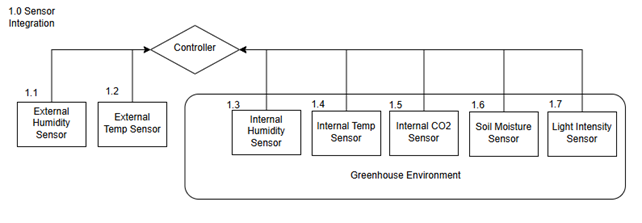
\includegraphics[width=0.8\textwidth]{figs/phys1.png}
    \caption{Sensor Physical Decomposition}
    \label{fig:sensor_decomposition}
\end{figure}

\begin{figure}[H]
    \centering
    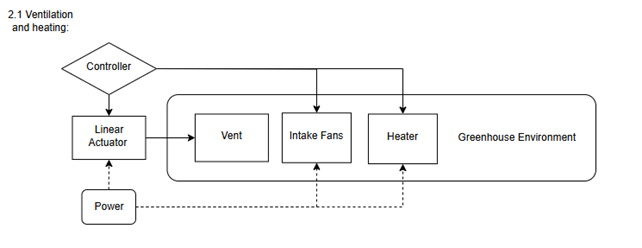
\includegraphics[width=0.8\textwidth]{figs/phys2.png}
    \caption{Ventilation Physical Decomposition}
    \label{fig:ventilation_decomposition}
\end{figure}

\begin{figure}[H]
    \centering
    \includegraphics[width=0.8\textwidth]{figs/phys3.png}
    \caption{Irrigation Physical Decomposition}
    \label{fig:irrigation_decomposition}
\end{figure}

\begin{figure}[H]
    \centering
    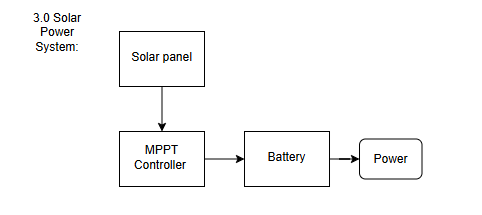
\includegraphics[width=0.8\textwidth]{figs/phys4.png}
    \caption{Solar Physical Decomposition}
    \label{fig:solar_decomposition}
\end{figure}







